\documentclass[12pt]{article}

\usepackage[margin=2.5cm, a4paper]{geometry} % Rand
\usepackage{setspace} % Zeilenabstand

\usepackage[utf8]{inputenc}
\usepackage[ngerman]{babel}
\usepackage{pdfpages}
\usepackage{epigraph}
\usepackage{xcolor}

\onehalfspacing % Zeilenabstand 1,5

\begin{document}

% \maketitle
% \thispagestyle{empty}
% \newpage

\begin{titlepage}
	\centering
	{\scshape\LARGE DHBW Karlsruhe\par}
	\vspace{1cm}
	{\scshape\Large Projekthandbuch\par}
	\vspace{1.5cm}
	{\huge\bfseries ClimateSight\par}
	\vspace{2cm}
	{\Large\itshape Leon Fertig (1142628)\\Matteo Kosina (2912404)\par}
	\vfill
	% \includegraphics[width=pagewidth]{Bilder/Titelbild.jpg}\par\vspace{1cm}
	\vfill

    % Bottom of the page
	{\large \today\par}
\end{titlepage}

\tableofcontents
\thispagestyle{empty}
\newpage

\setcounter{page}{1}

\section{Einführung}
Wir - das Team des Projekts {\bf ClimateSight} - haben im Rahmen der Vorlesung {\it Web-Engineering I} bei Herrn Jürgen Röthig eine Webseite entwickelt und begleitend zu dieser Webseite dieses Projekthandbuch über die Planung und organisatorische Steuerung unseres Projektes erstellt.\
Alle Planungsdokumente wurde erstellt, \underline{nachdem} ein Projektmitglied die Gruppe verlassen hat, sodass dieser Verlust keine relevanten Auswirkungen auf das Projekt hatte.

\section{Projektvorstellung}
{\color{red} kurze Projektvorstellung (README)}

\section{Protokolle}
Für die Protokollierung ist eine Vorlage entworfen worden, nach der die Treffen jeweils protokolliert worden sind. Zwei Beispiele finden sich nachfolgend.
\newline
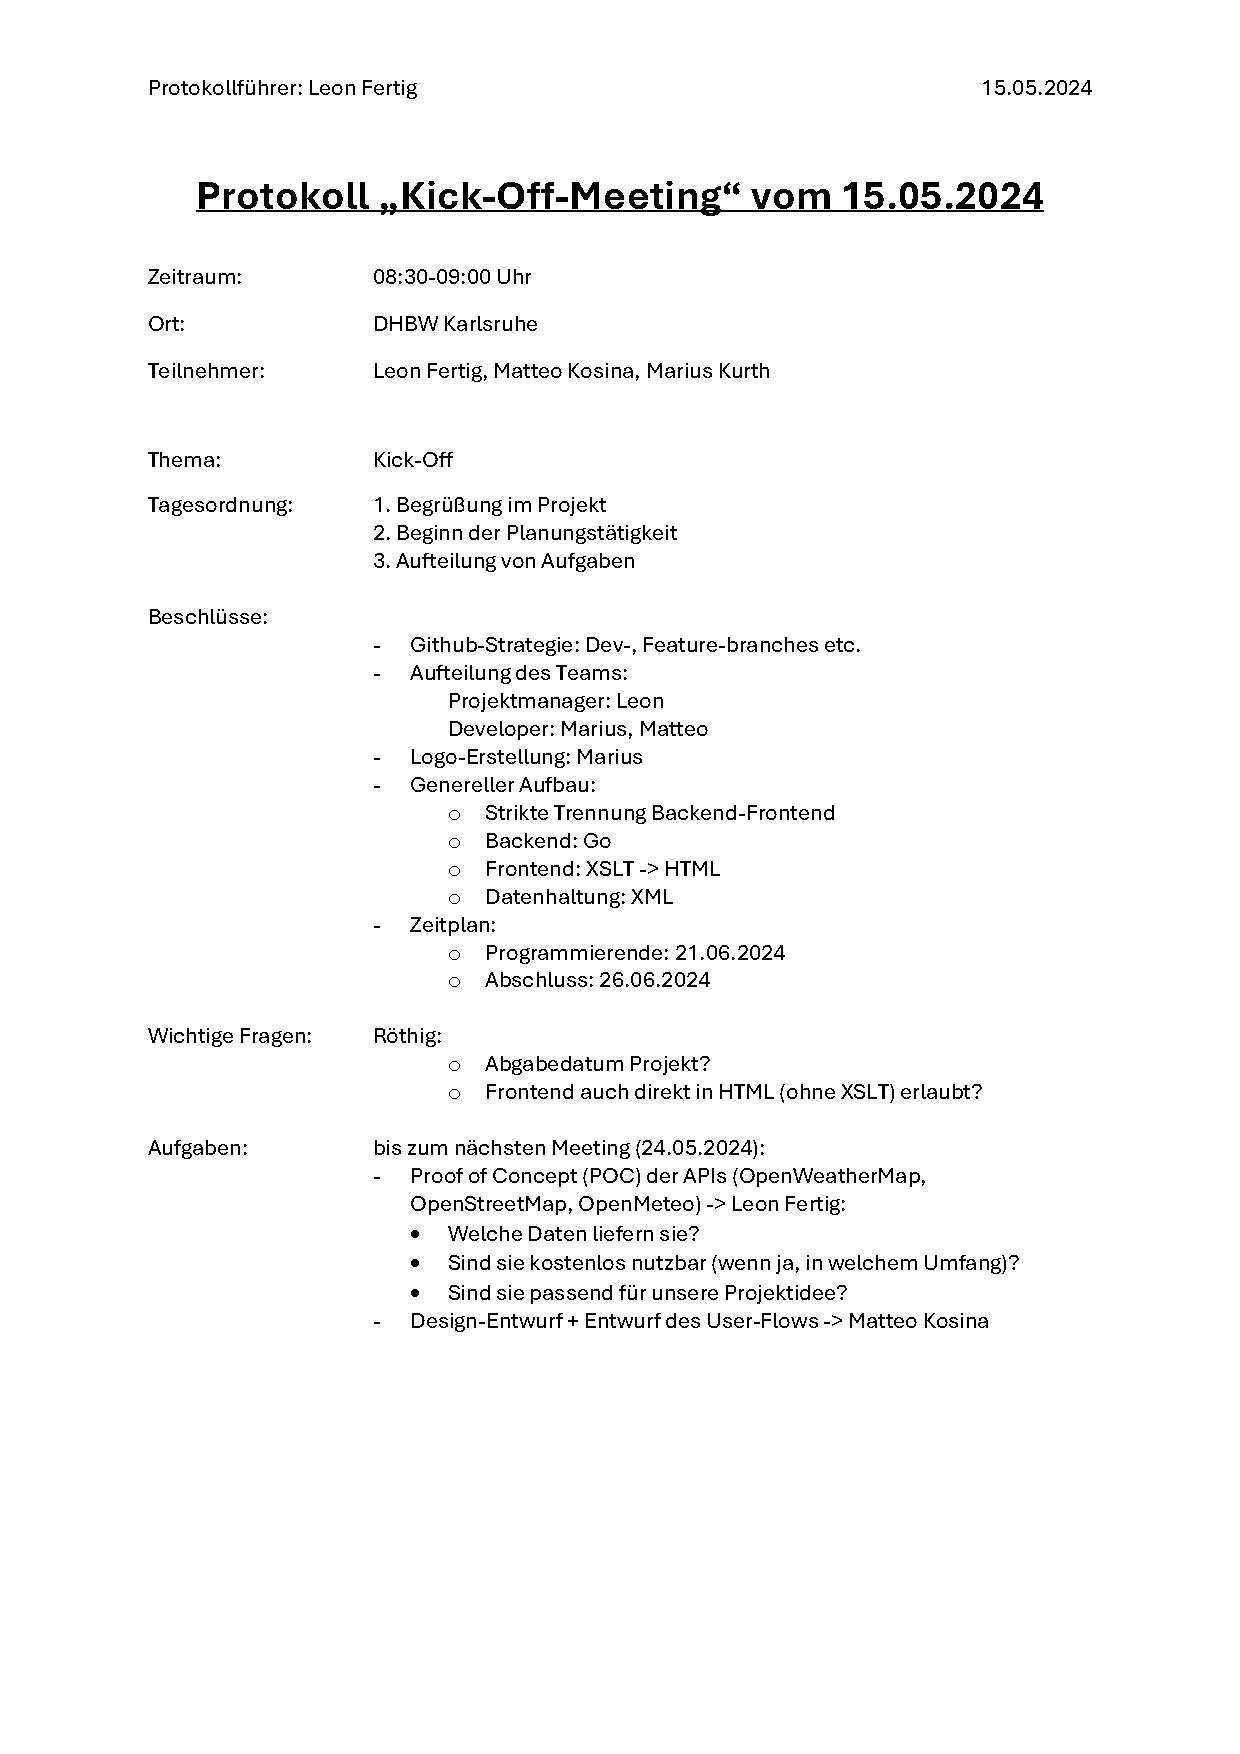
\includegraphics[width=\textwidth]{Planungsdokumente/graphics/Protokoll1.pdf}
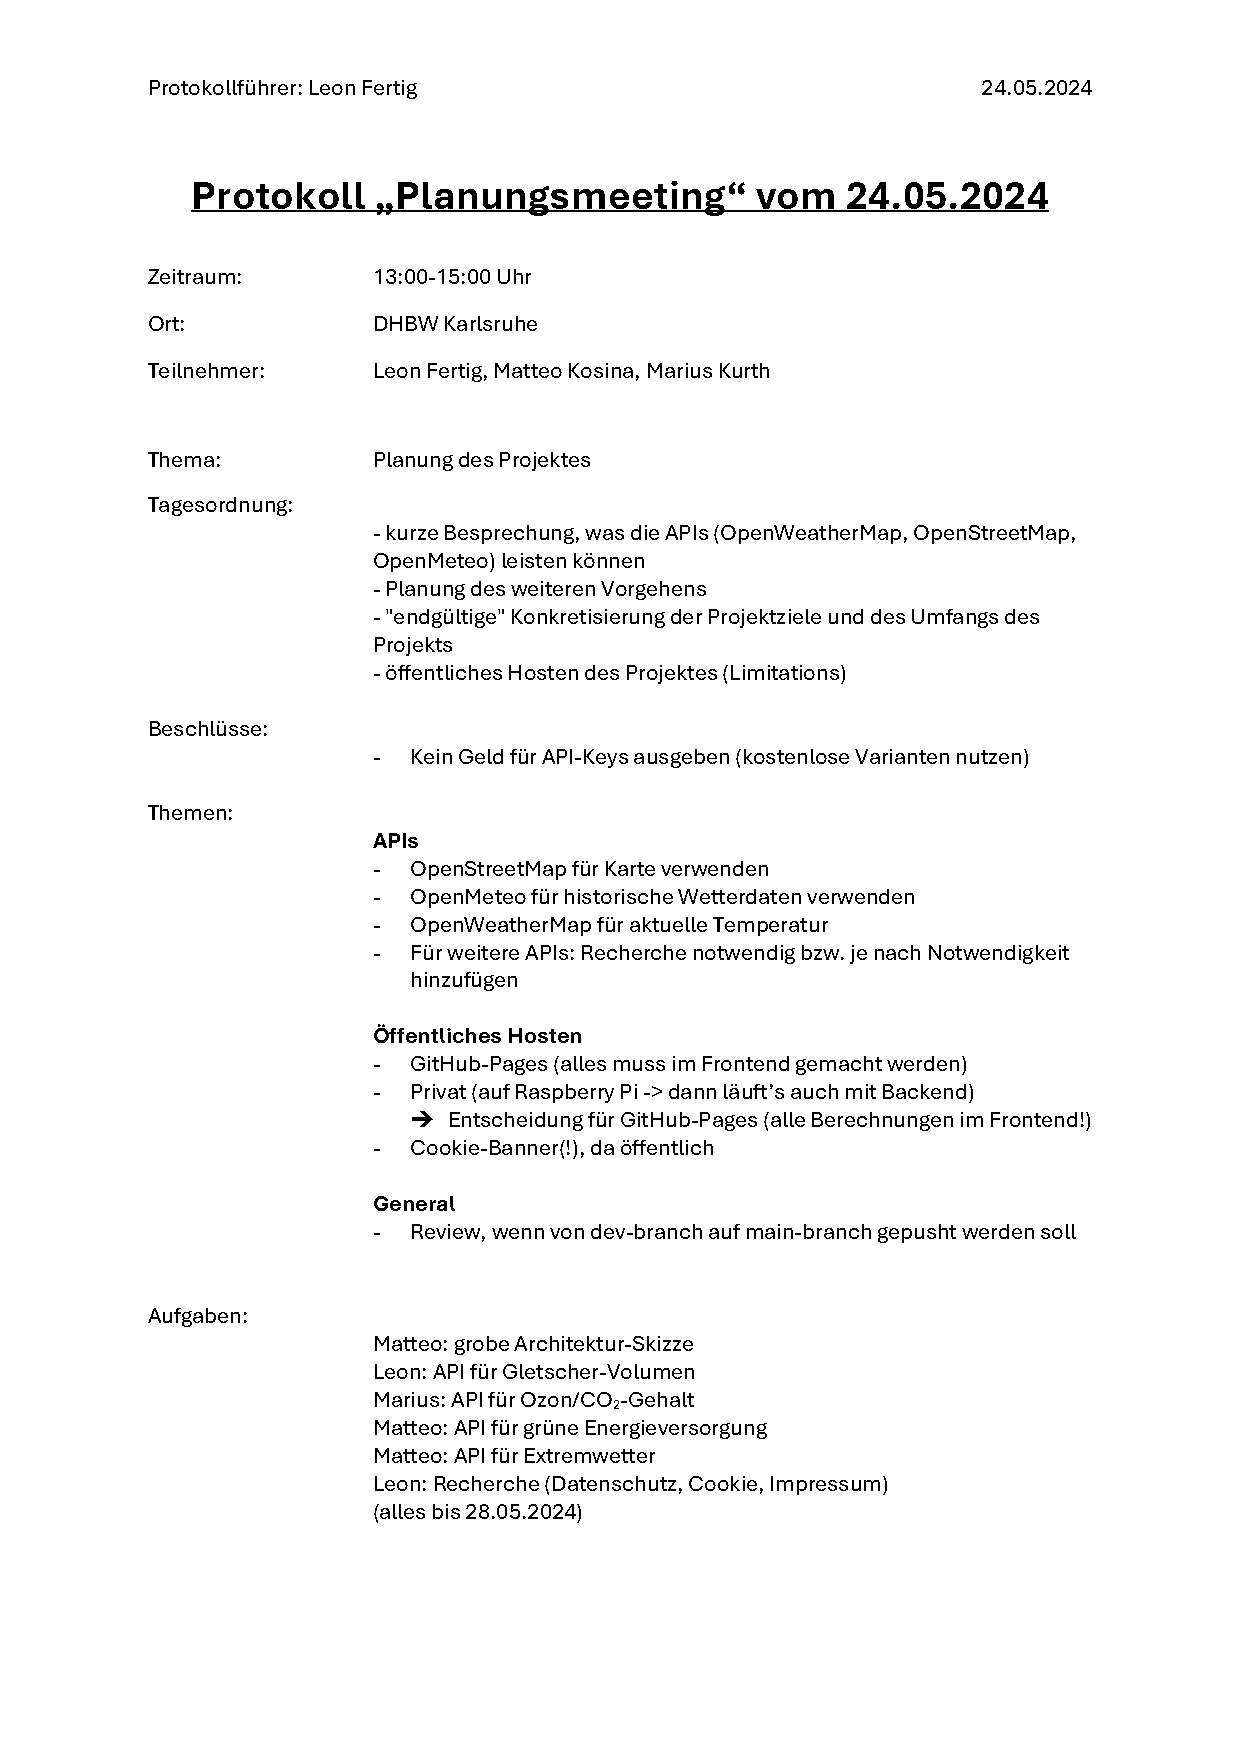
\includegraphics[width=\textwidth]{Planungsdokumente/graphics/Protokoll2.pdf}

\section{Projektauftrag}
Der Projektauftrag geht aus den Anforderungen des Auftraggebers Herrn Röthig hervor und gibt wieder, was der Auftraggeber von uns erwartet. Das Projektgesamtziel, die Teilziele und die Rahmenbedingungen und der Projektkontext sind direkt aus den Anforderungen von Herrn Röthig zitiert.
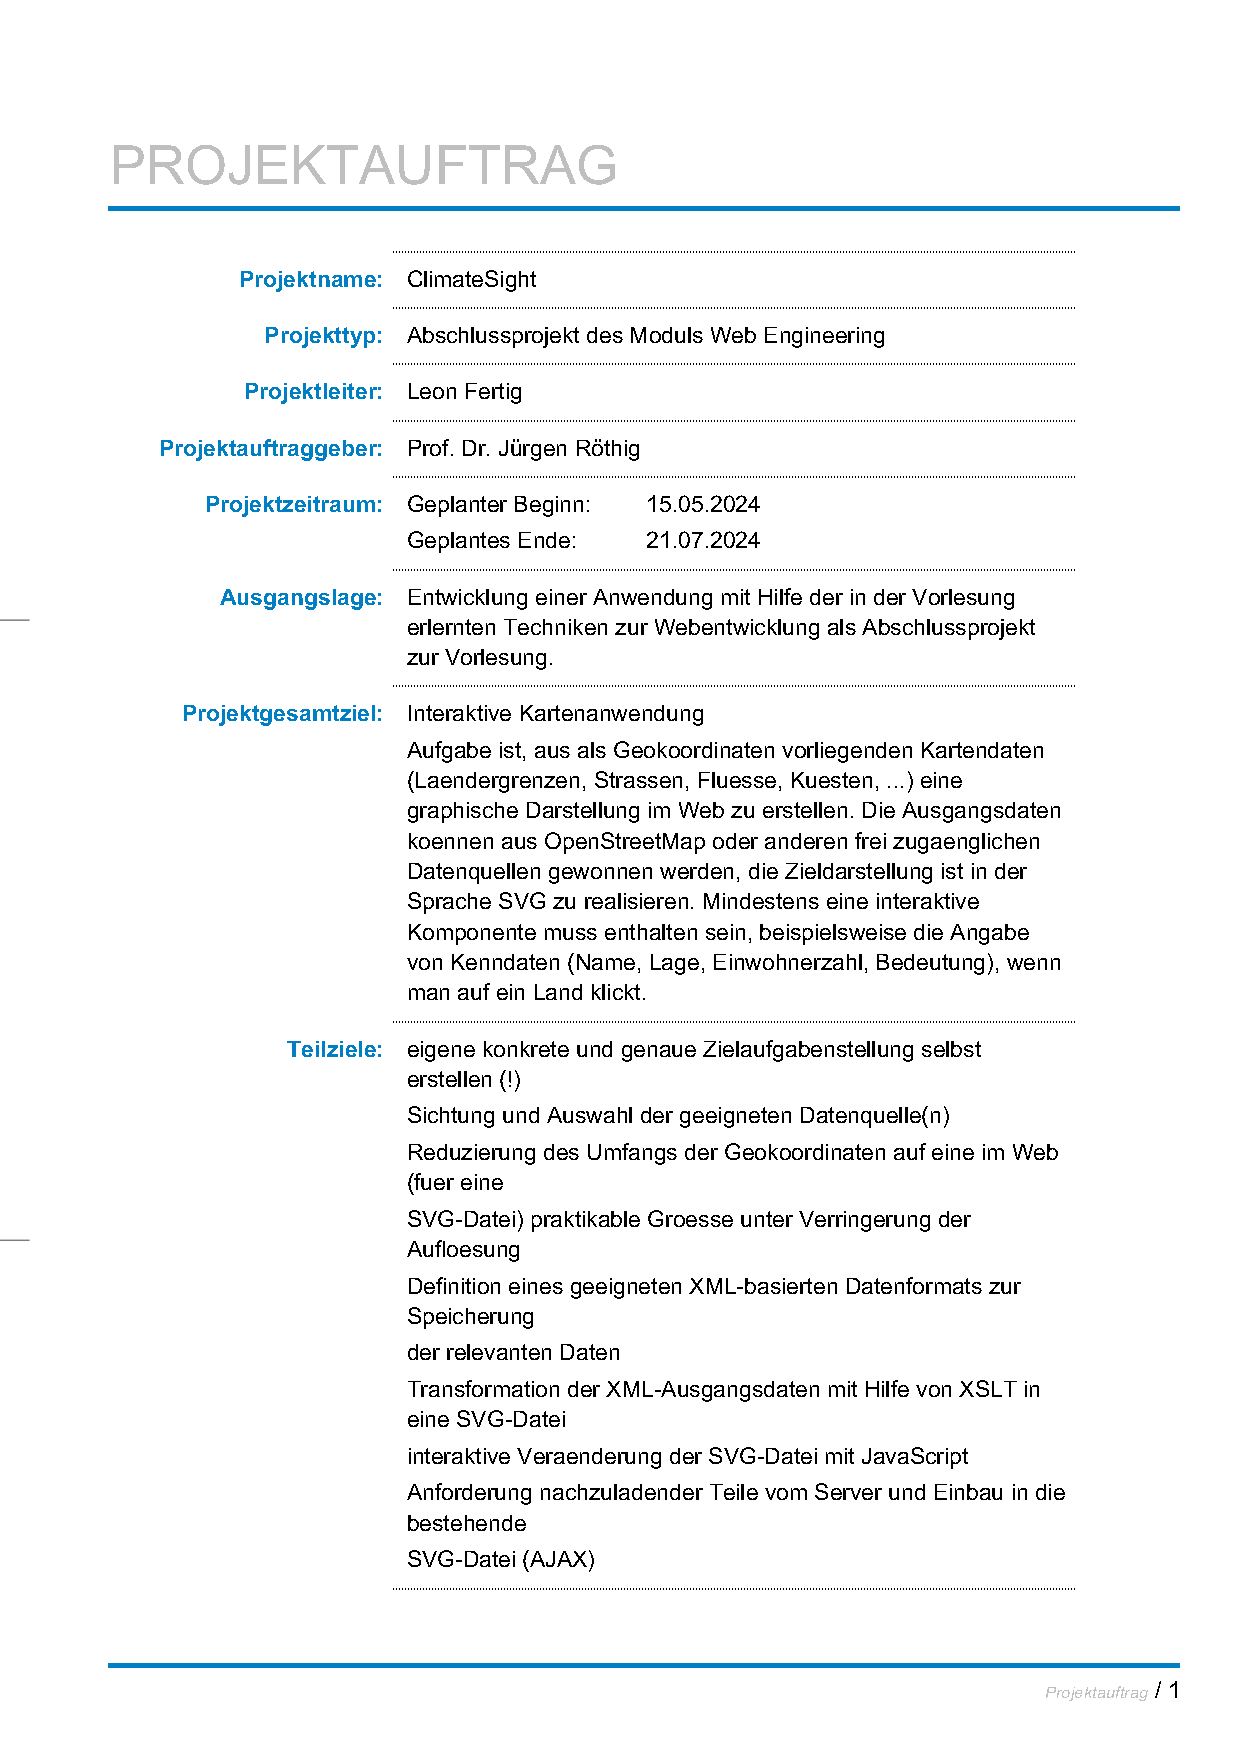
\includepdf[pages=-]{Planungsdokumente/graphics/Projektauftrag.pdf}

\section{Projektziele}
\subsection*{Muss-Kriterien}
\begin{itemize}
    \item Entwicklung einer Web-Applikation für Desktop-PCs
    \item Start-Seite
    \item Sprache-Einstellungen für Deutsch und Englisch
    \item Weltkarte, die die einzelnen Länder interaktiv mit Informationen verknüpft. Bei Klicken über ein Land erscheinen verschiedene Informationen:
    \begin{itemize}
        \item durchschnittliche Jahrestemperatur (inkl. historische Daten)
        \item Niederschlag pro m$^2$
        \item UV-Einstrahlung
        \item historische Wetterdaten
    \end{itemize}
    \item ausführliche Installationsanleitung
\end{itemize}

\subsection*{Soll-Kriterien}
\begin{itemize}
    \item lokale Nachrichten (mit Fokus auf Klima + Wetter)
    \item Klimafilter (nach Temperatur und/oder Niederschlag)
    \item Anzeige von aktueller Temperatur
\end{itemize}

\subsection*{Kann-Kriterien}
\begin{itemize}
    \item verschiedene Kartenansichten: Satellit, geographisch, Heat-Map
    \item lokale Wetterkarten
\end{itemize}

\subsection*{Abgrenzungskriterien}
\begin{itemize}
    \item kein Einsatz von KI
    \item keine Routenführung
    \item keine mobile Anwendung (nicht für Smartphone oder Tablets optimiert)
\end{itemize}

\section{Phasen- und Meilensteinplan}
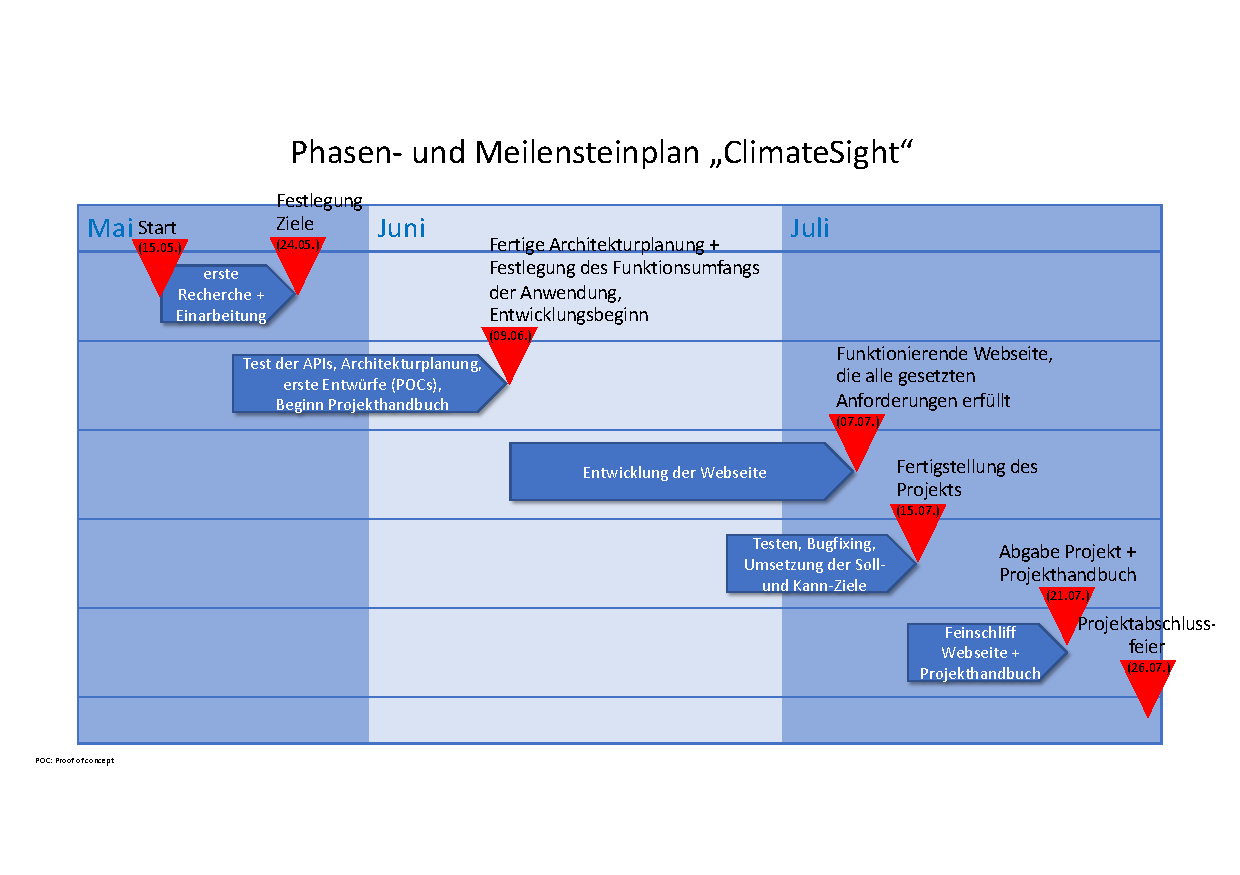
\includegraphics[width=\textwidth]{Planungsdokumente/graphics/Meilensteinplan.pdf}

\section{Projektorganigramm}
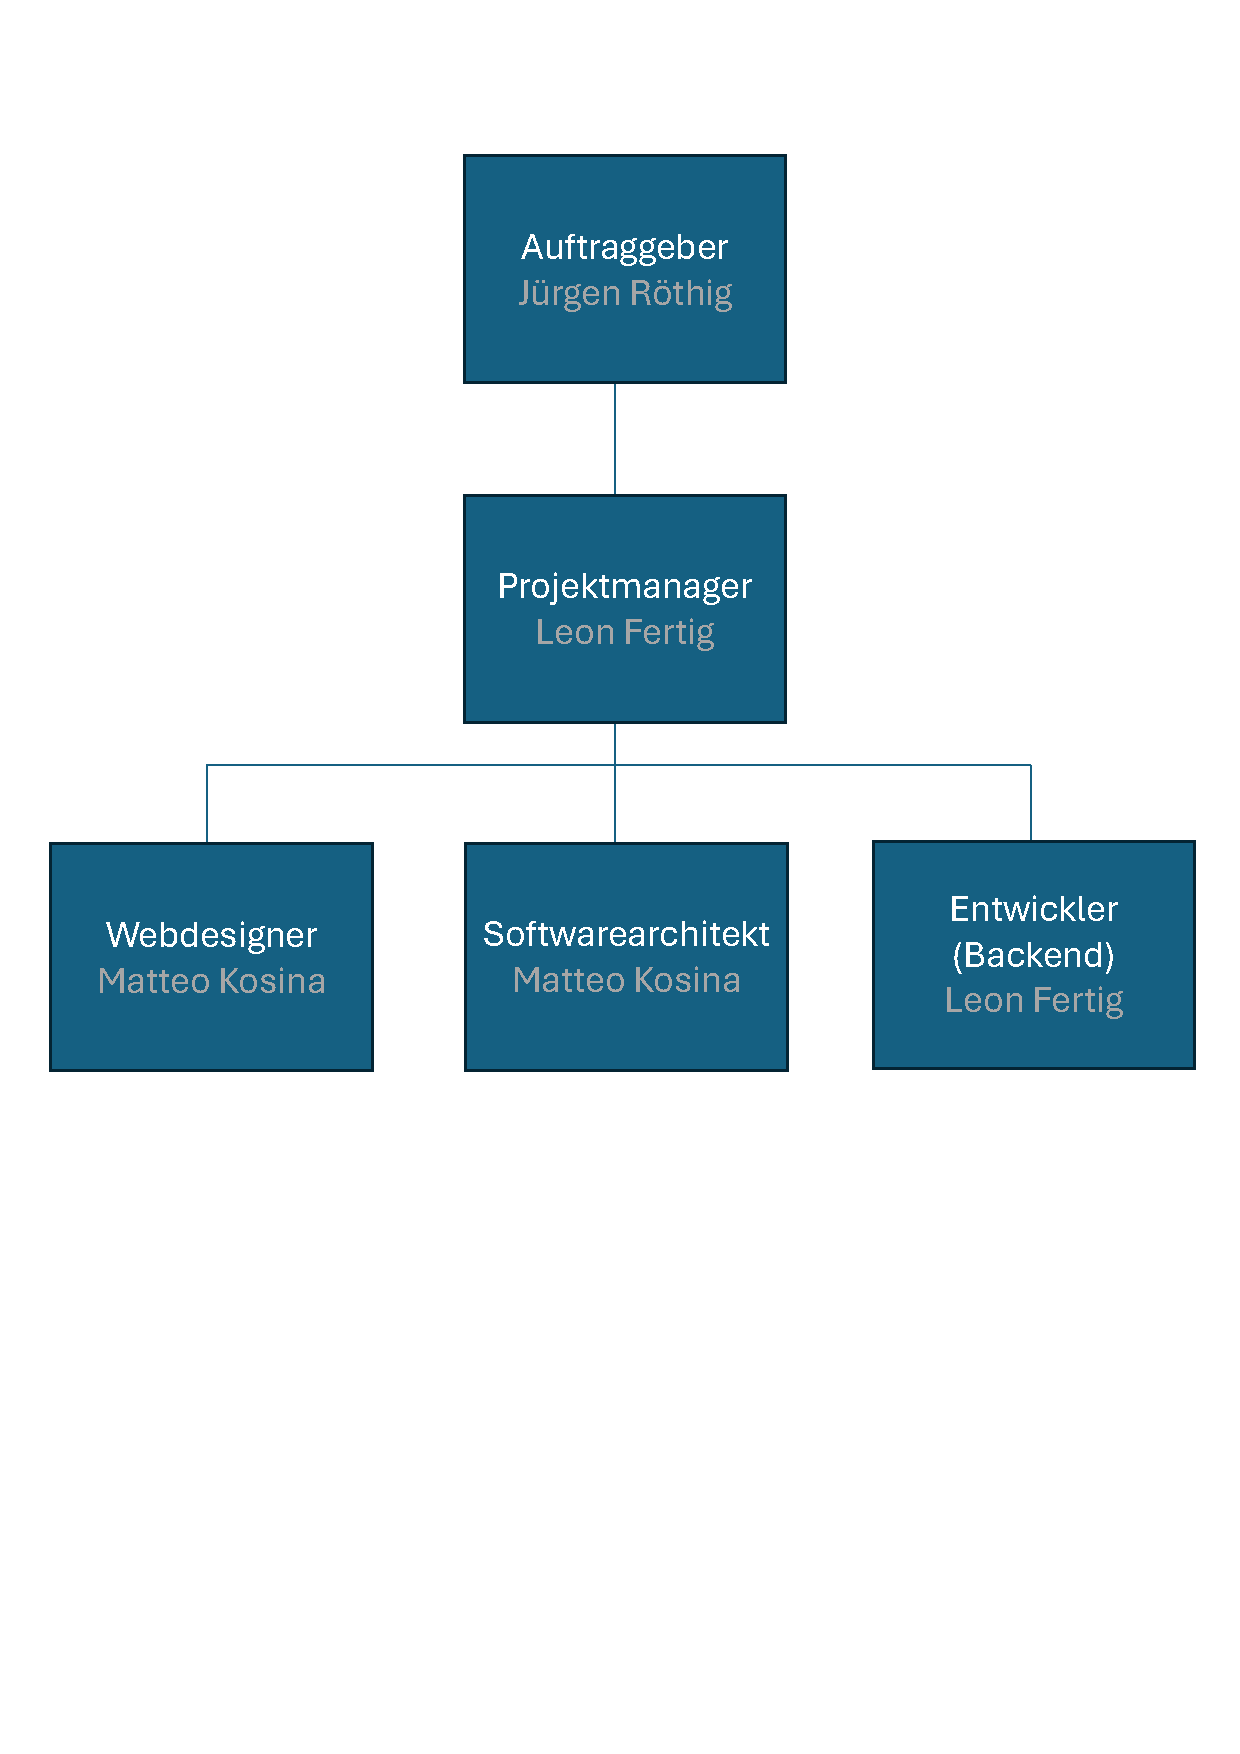
\includegraphics[width=\textwidth]{Planungsdokumente/graphics/Projektorganigramm.pdf}

\section{Offene-Punkte-Liste OPL}
Offene Punkteliste zum 04.06.2024.
\newline
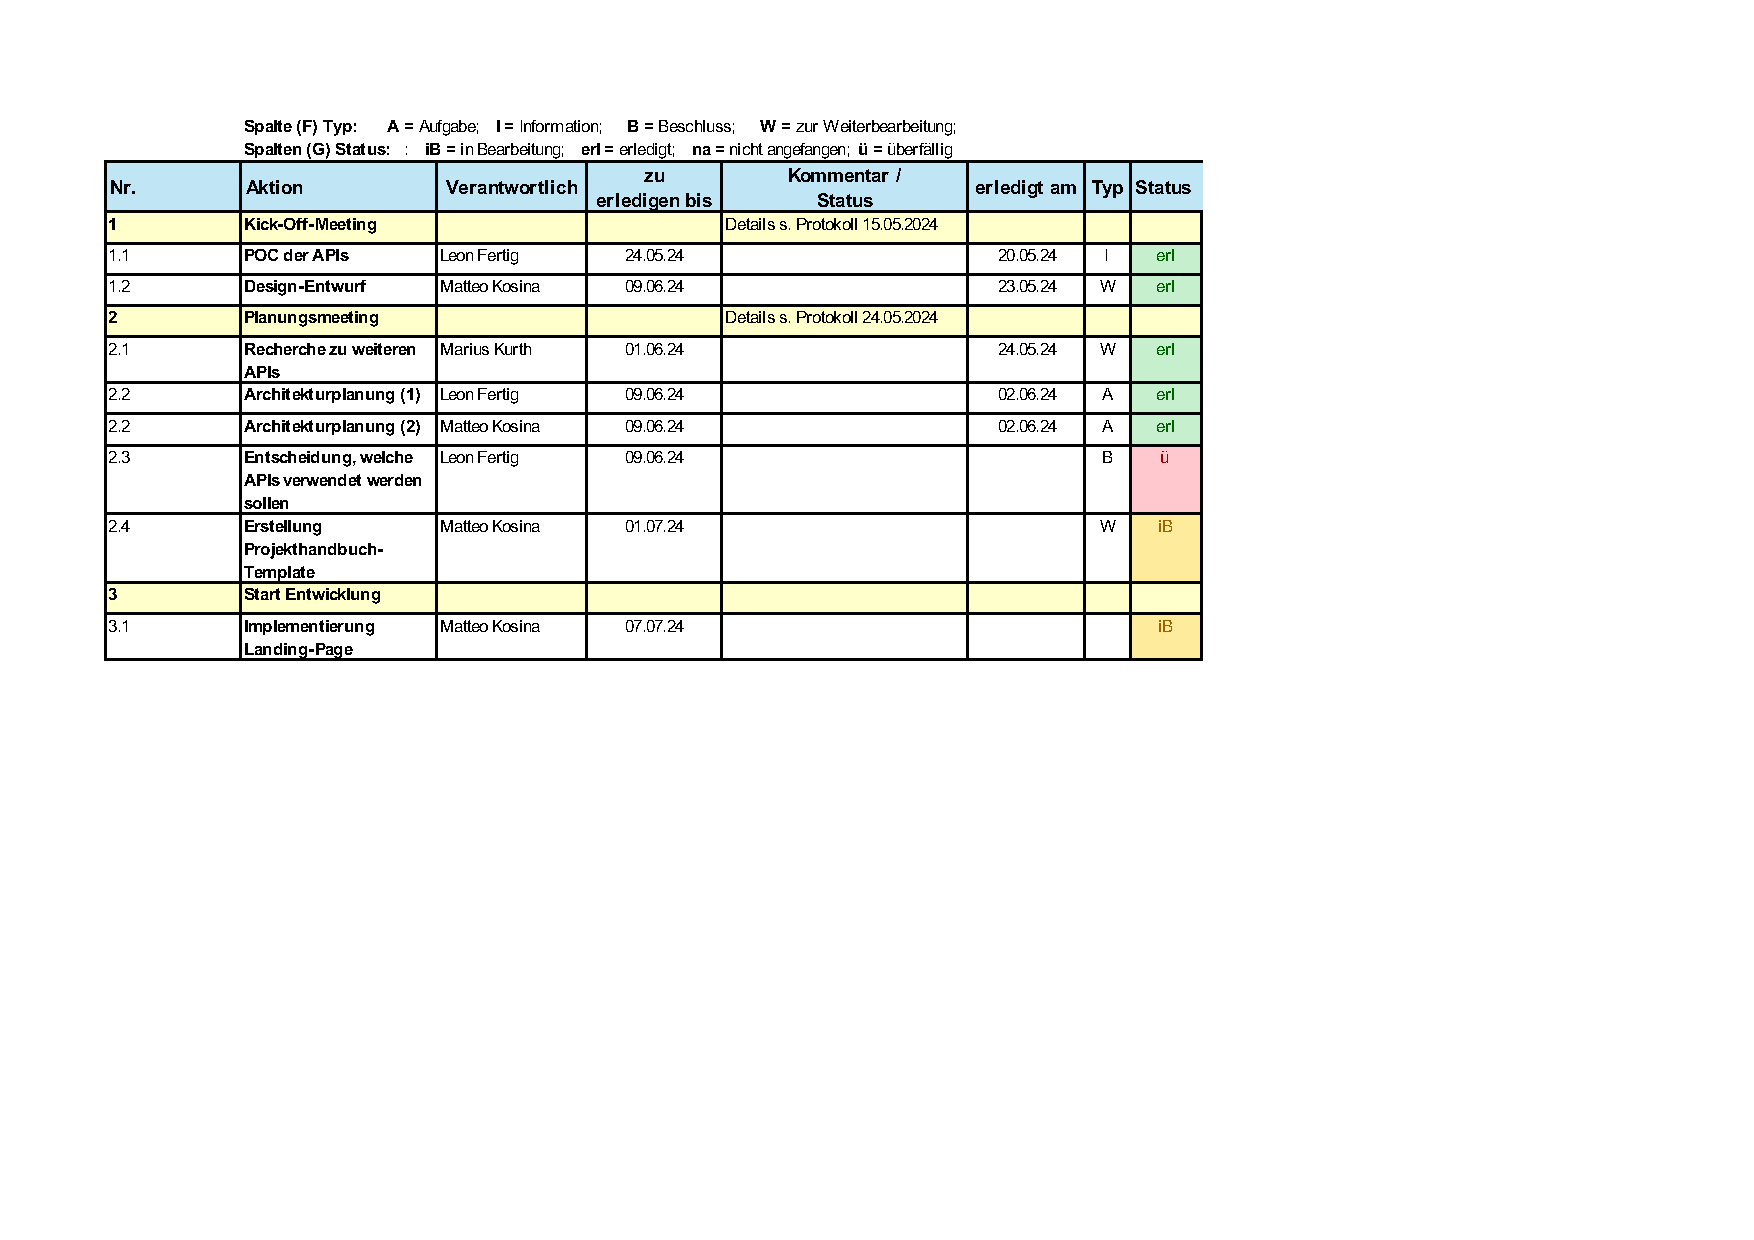
\includegraphics[width=\textwidth]{Planungsdokumente/graphics/Offene_Punkteliste.pdf}

\section{Projektstrukturplan}
Es wurde eine Gemischter Projektstrukturplan erstellt:
\begin{itemize}
	\item {\bf Projektmanagement}: Mischung aus Objektorientierung und Phasenorientierung
	\item {\bf Frontend}: Objektorientierung (wobei die Überarbeitung von UX + Design eher einem phasenorientierten Ansatz entspricht)
	\item {\bf Backend}: phasenorientiert
\end{itemize}
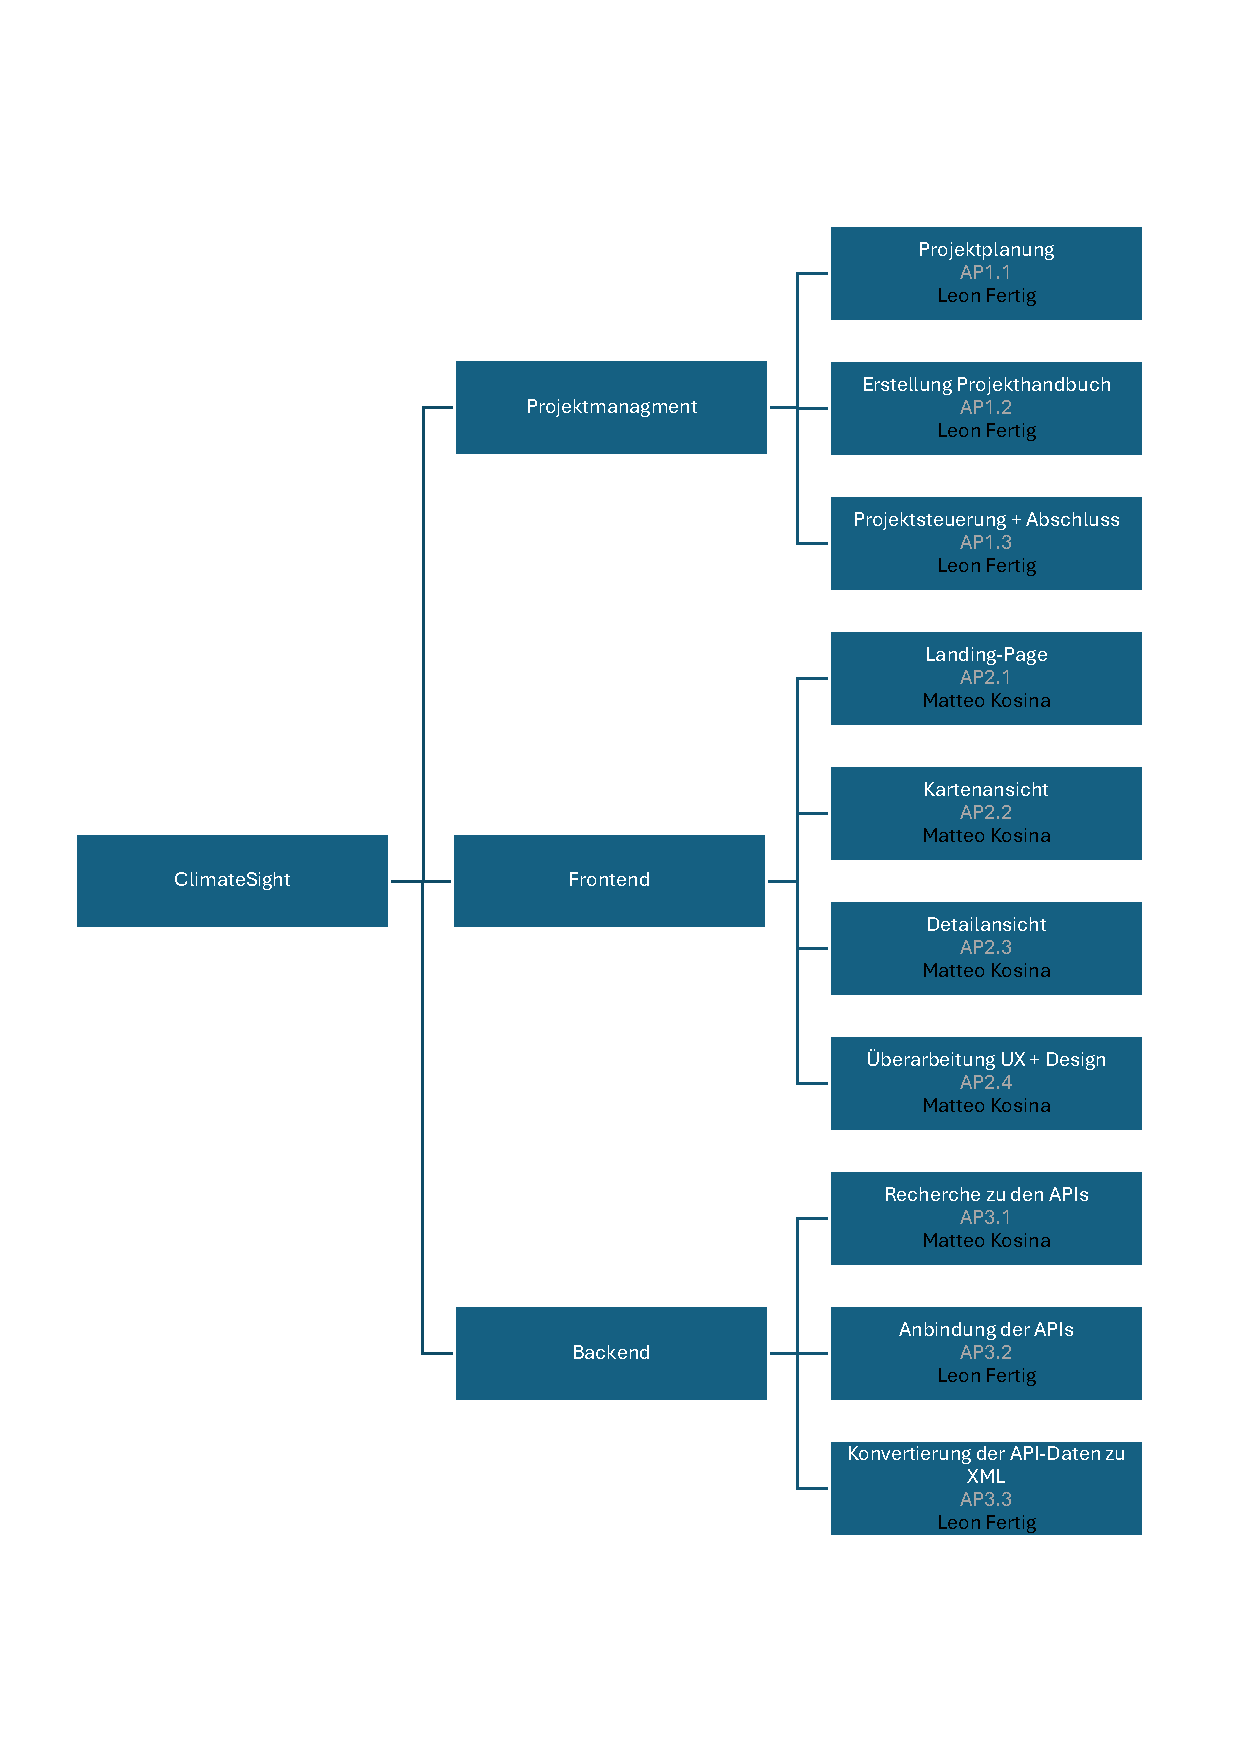
\includegraphics[width=\textwidth]{Planungsdokumente/graphics/Projektstrukturplan.pdf}

\section{Arbeitspaketbeschreibungen}
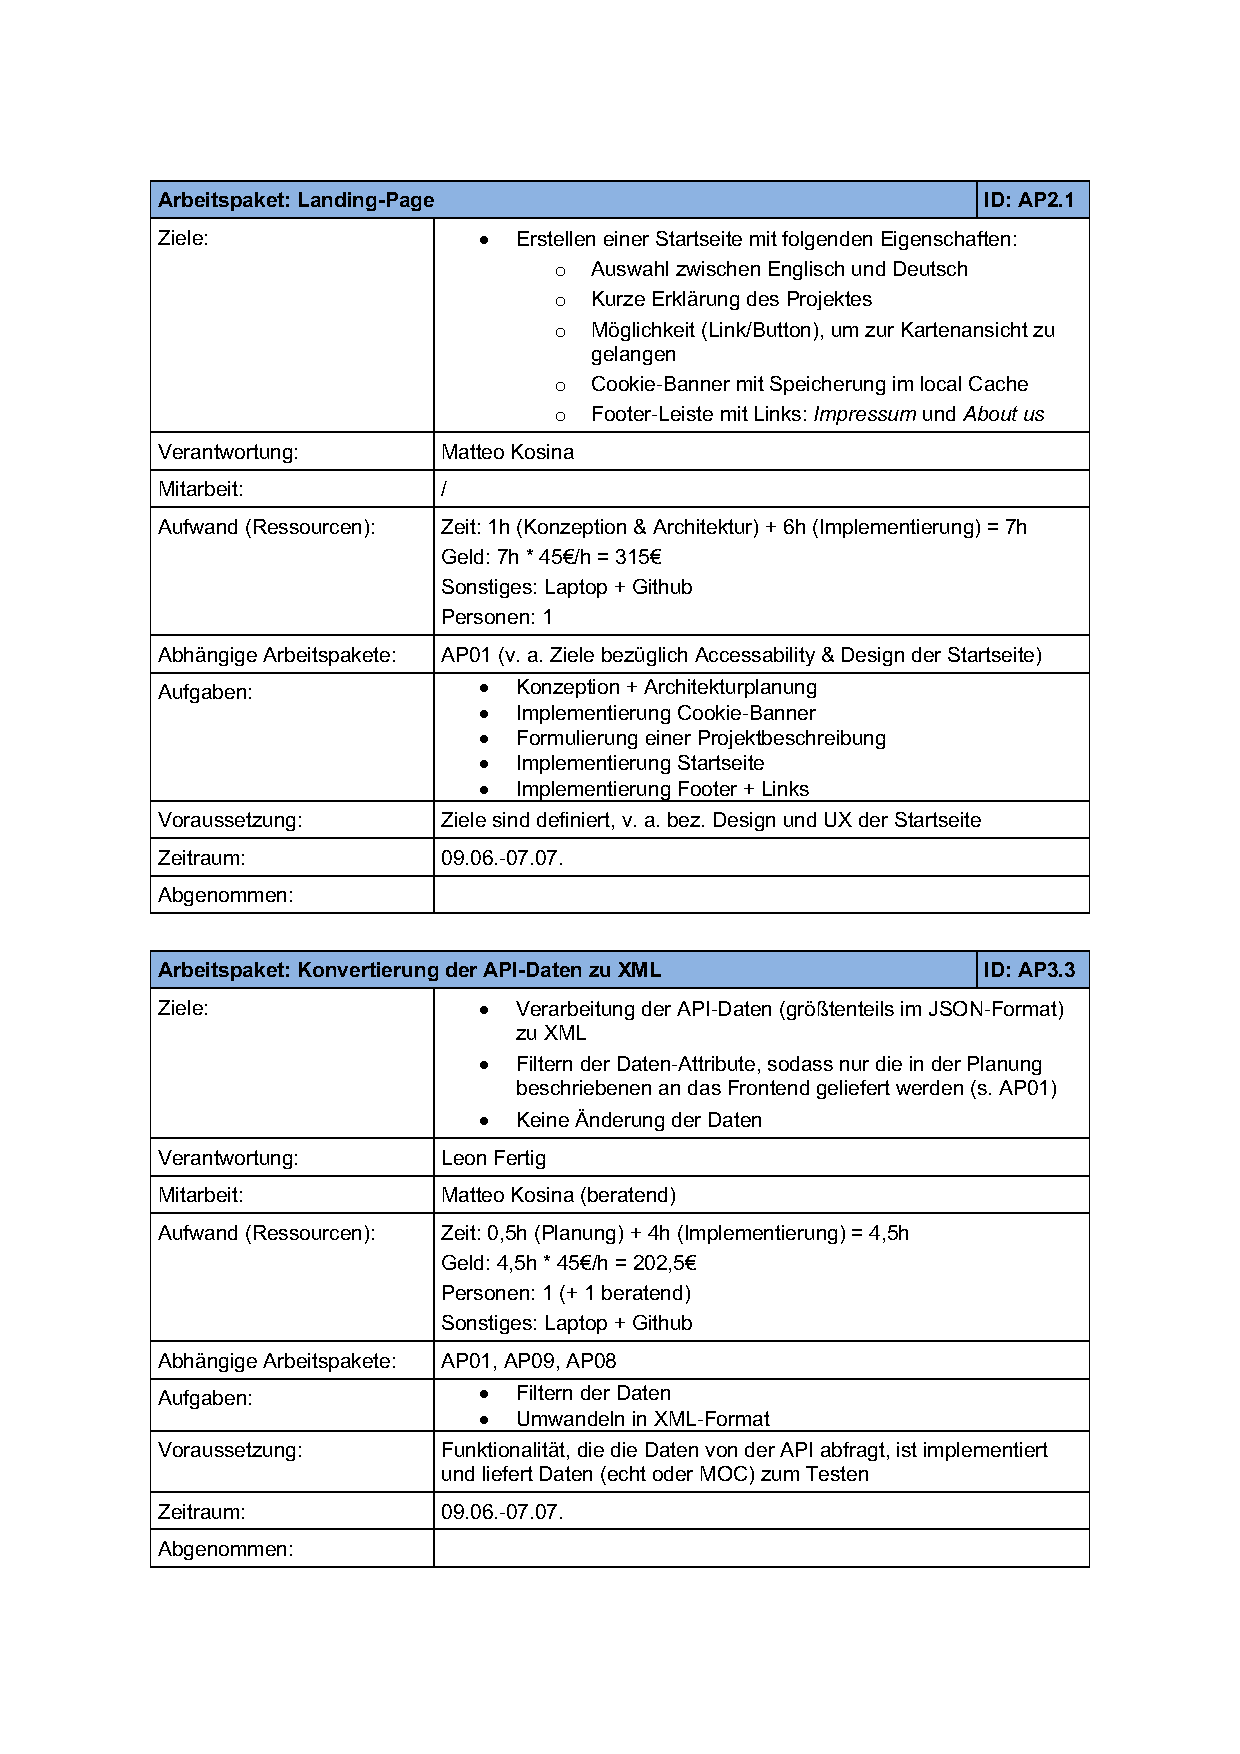
\includegraphics[width=\textwidth]{Planungsdokumente/graphics/Arbeitspakete.pdf}

\section{Projektablaufplan}
{\color{red} brauchen wir das oder ist das im Gantt-Diagramm in ausführlicher Form enthalten?!}

\section{Gantt-Diagramm}
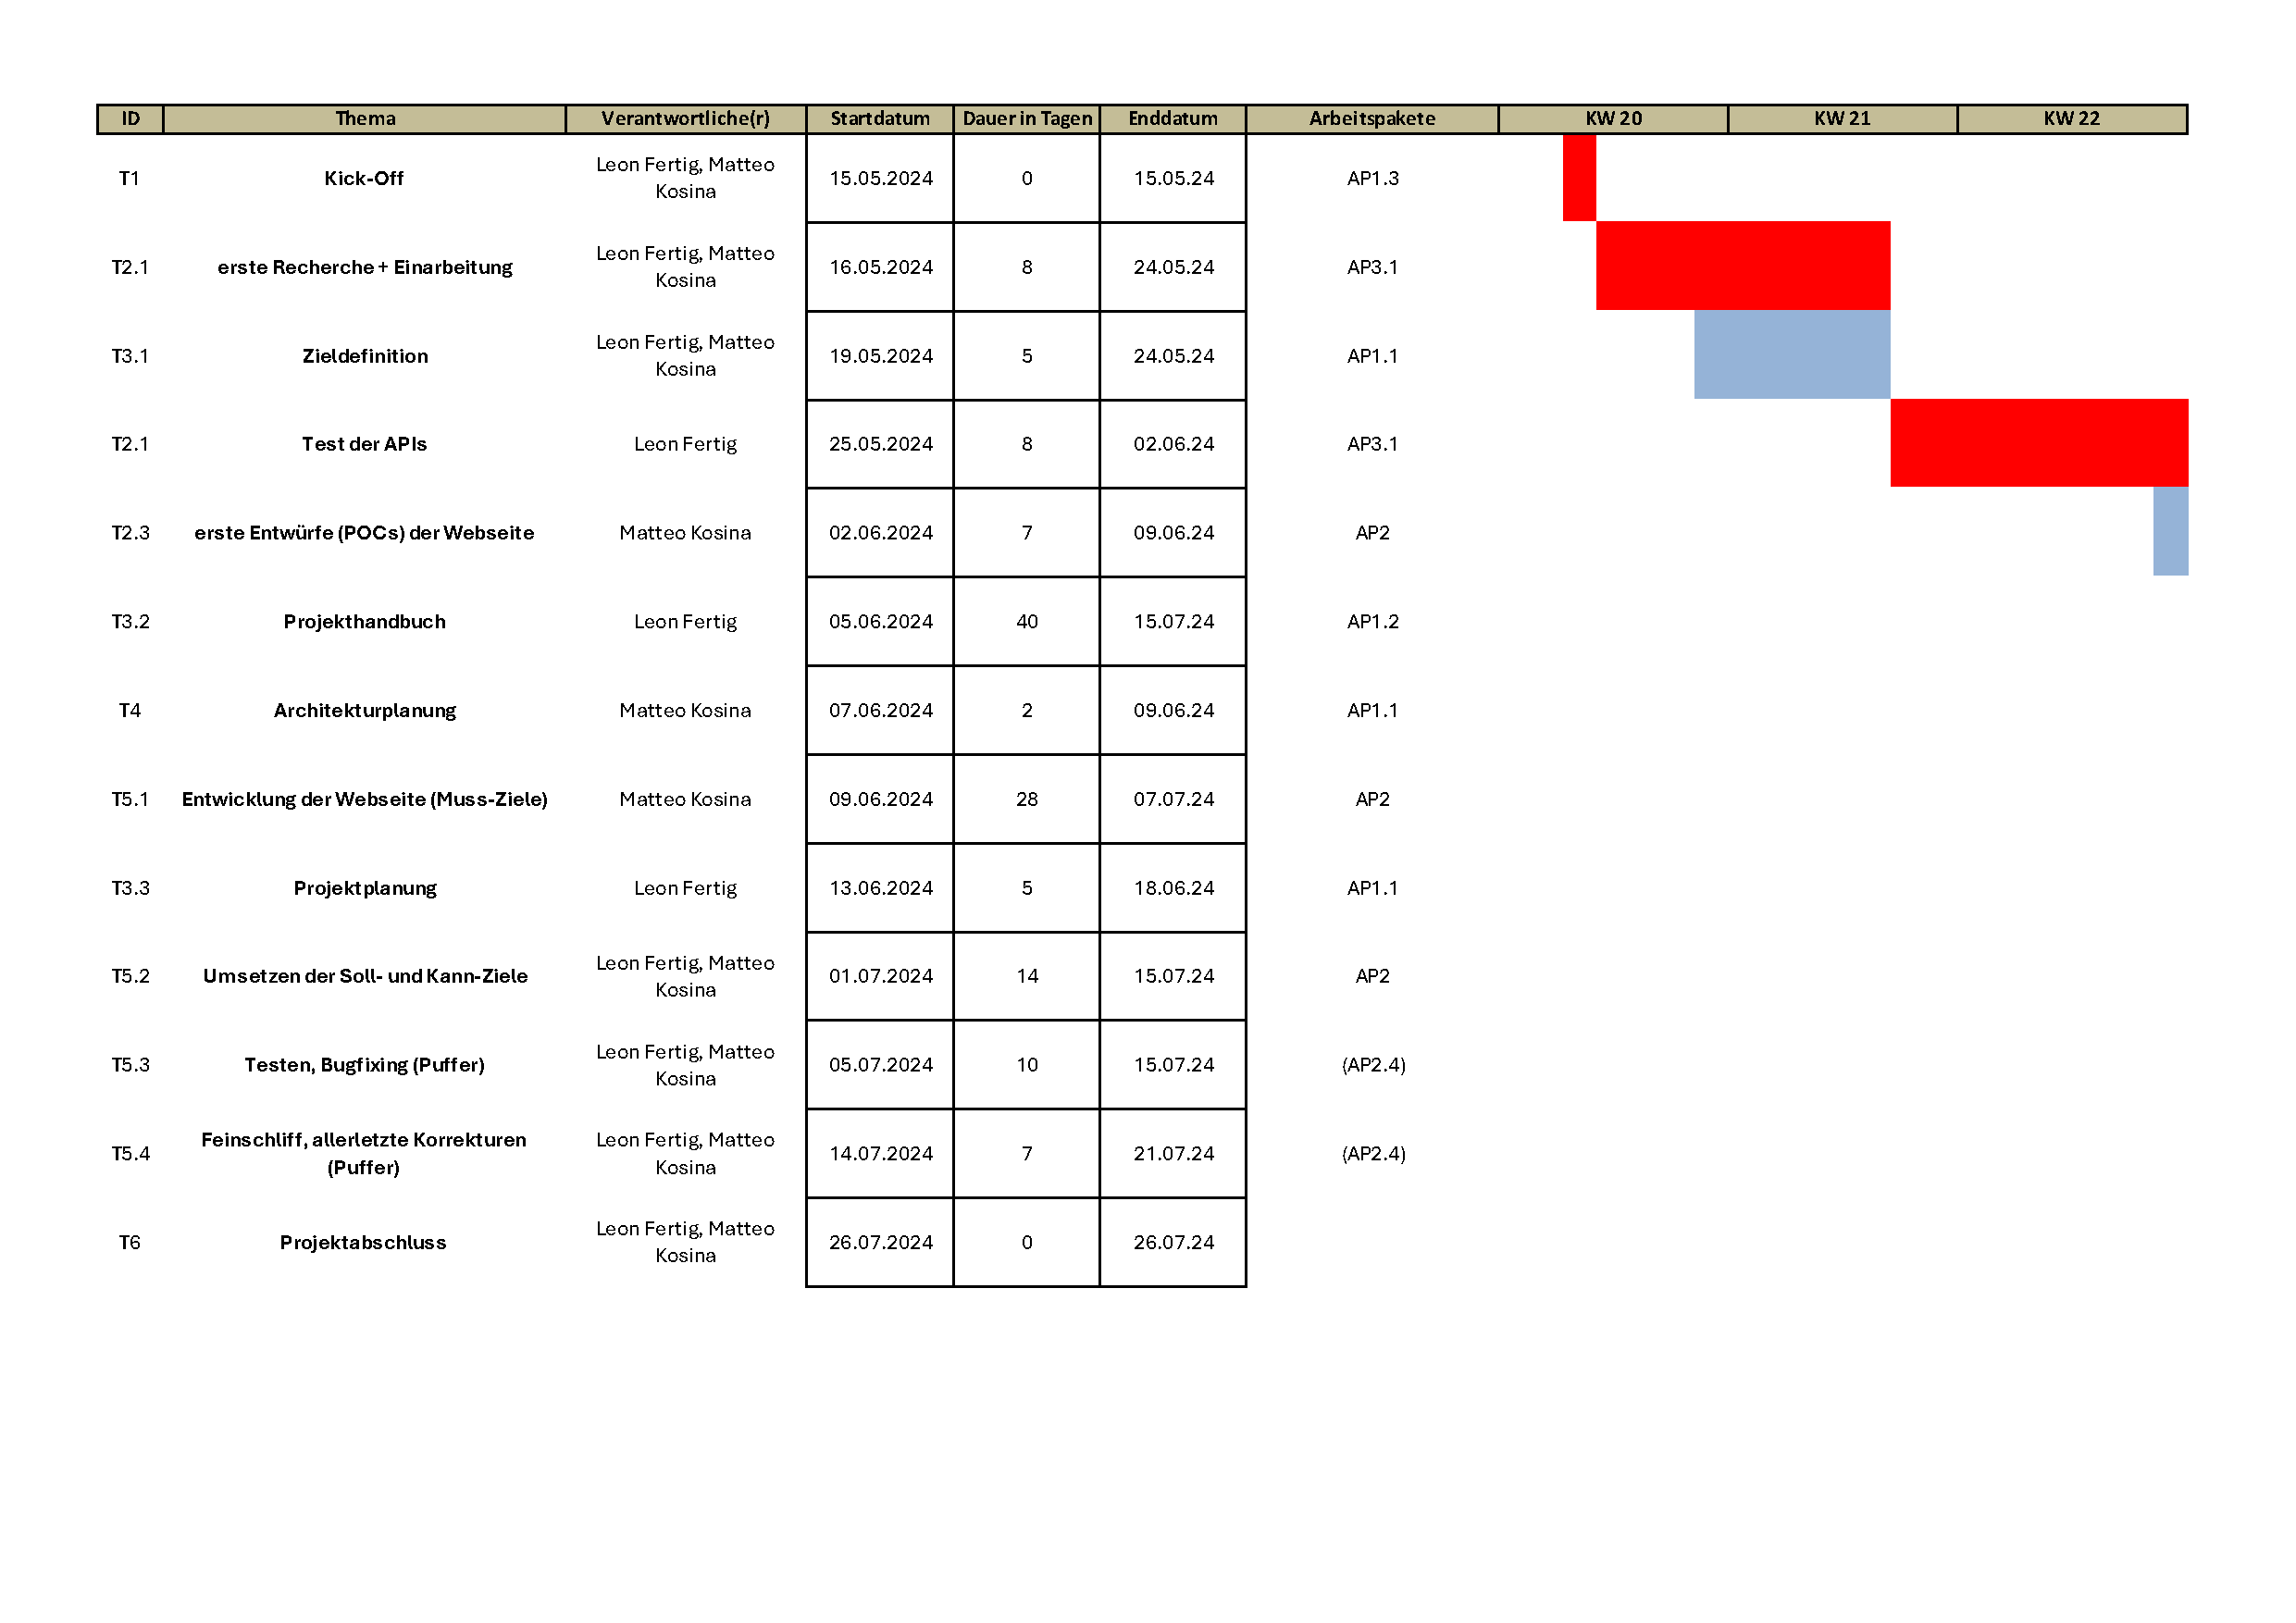
\includegraphics[width=\textwidth, page=1]{Planungsdokumente/graphics/Gantt_Diagramm.pdf}
\includegraphics[width=\textwidth, page=2]{Planungsdokumente/graphics/Gantt_Diagramm.pdf}

\section{Projektplanung (Ressourcen, Kosten, Risiko, Stakeholder)}
Auf Basis der Arbeitspakete eine Ressourcenplanung und eine Kostenplanung erstellen.\\
Analog: Kostengang und Kostensumme erarbeiten\\
Risikoanalyse
\begin{itemize}
	\item Zeigen auf, welche Arten von Risiken Sie identifiziert haben
	\item Wie ist ihre Risikomatrix ausgestaltet?
	\item Erläutern Sie anhand ausgesuchter Beispiele, warum Sie eine bestimmte Art der Risikobehandlung ausgewählt haben (z.B. Vermeidung oder Verlagerung)
\item Entscheiden Sie frei zwischen einer quantitativen und qualitativen Risikobewertung
\end{itemize}
Stakeholderanalyse
\begin{itemize}
	\item Erstellen Sie eine geeignete Vorlage, definieren Sie die Parameter
	\item Führen Sie beispielhaft einige Stakeholderanalyse durch
\end{itemize}

\section{Ressourcen- und Kostenplan}
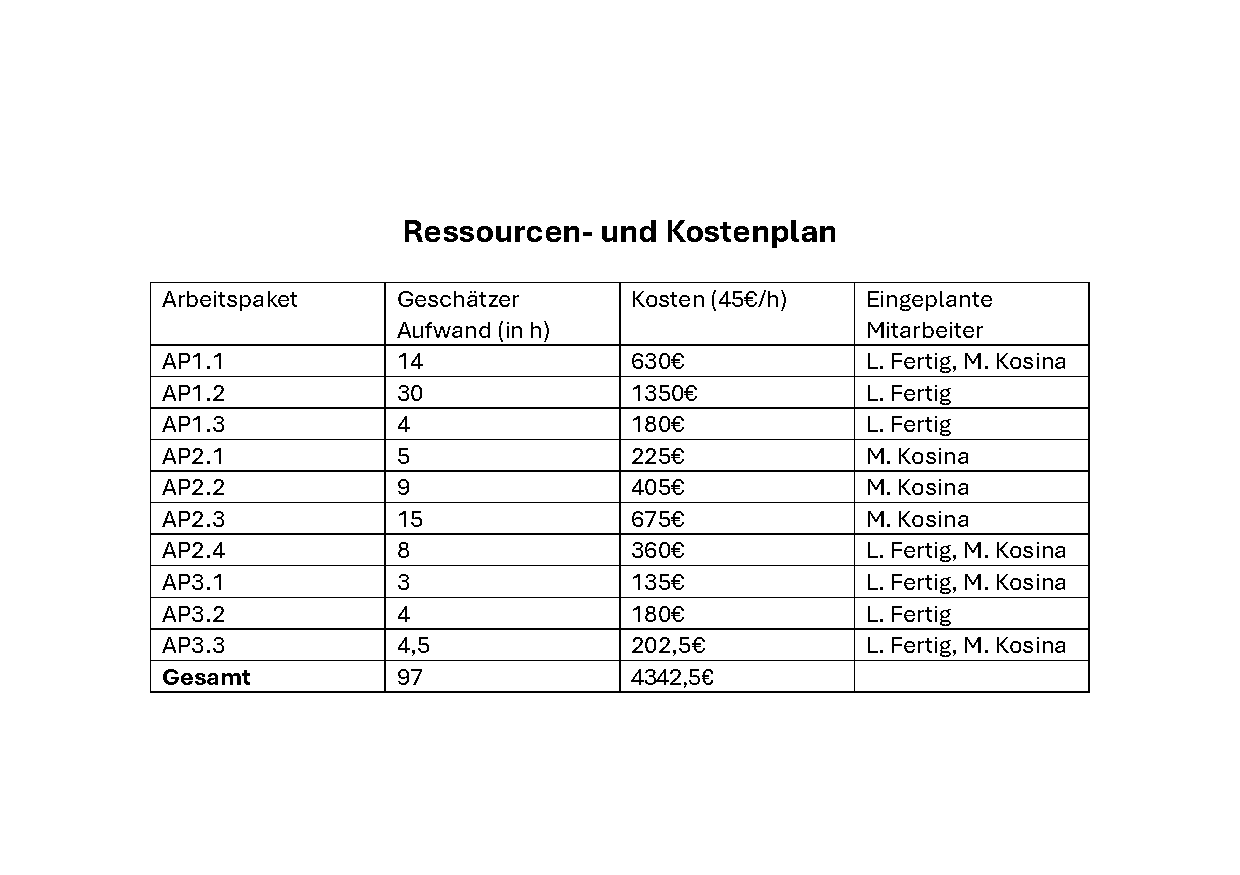
\includegraphics[width=\textwidth]{Planungsdokumente/graphics/Ressourcenplan.pdf}

\section{Risikoanalyse}
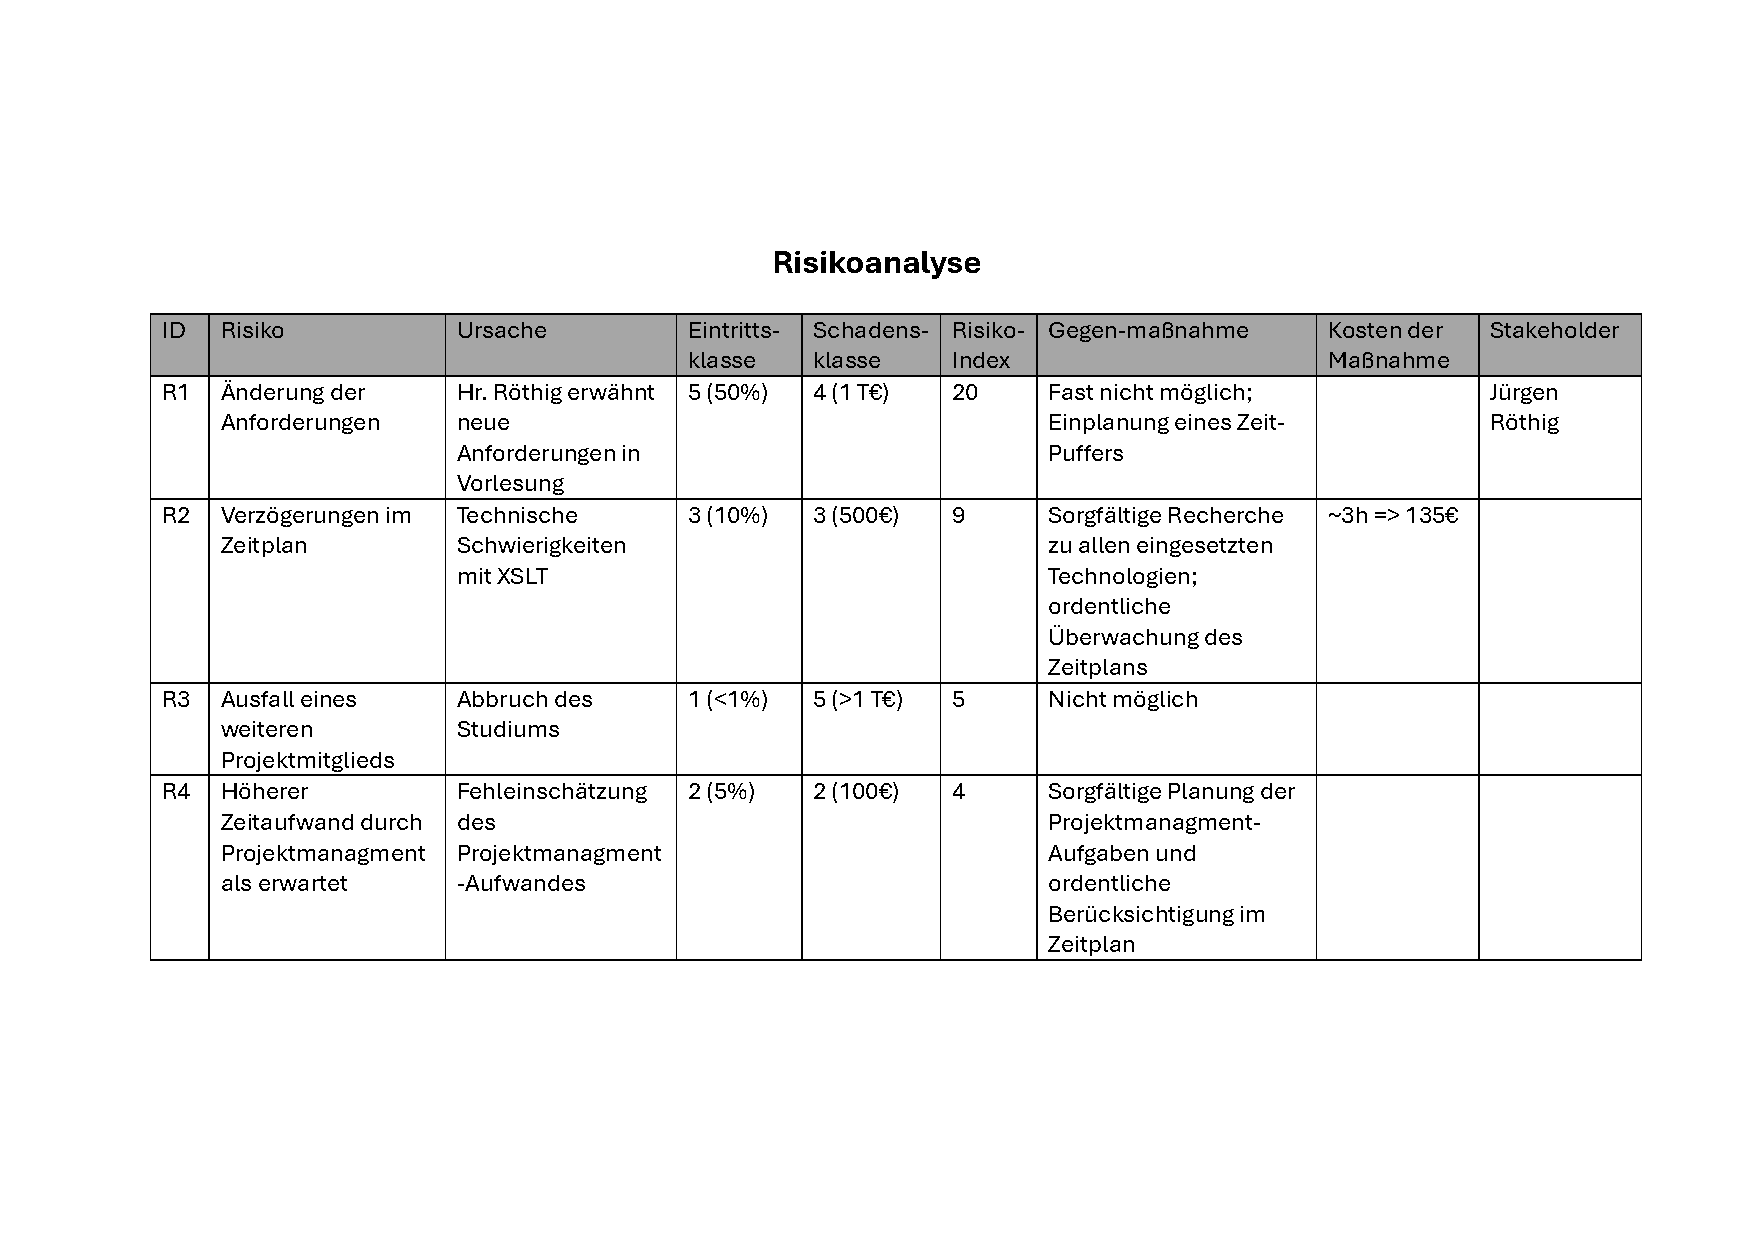
\includegraphics[width=\textwidth]{Planungsdokumente/graphics/Risikoanalyse.pdf}
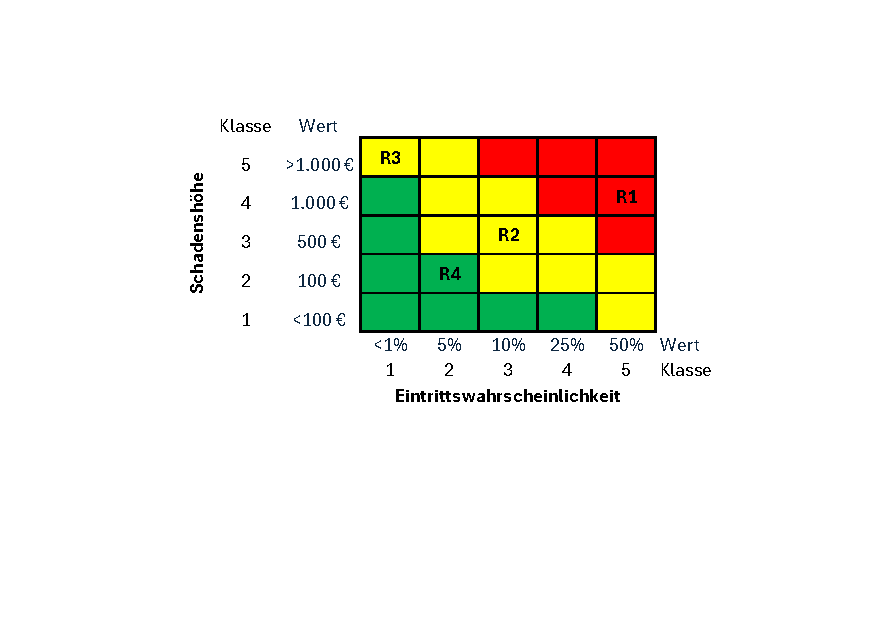
\includegraphics[width=\textwidth]{Planungsdokumente/graphics/Risikomatrix.pdf}

\section{Stakeholderanalyse}

\section{Projektstatusbericht}
Statusbericht (etwa in der Hälfte des Projektzeitraumes)

\section{Product Backlog und Sprint Backlog}
Einen Product Backlog
\begin{itemize}
	\item Es sollten mindestens vier bis fünf User Stories enthalten sein
	\item Fügen Sie auch ein Epic Beispiel ein
\end{itemize}
Sprint Backlog

→ Es sollten mindestens vier bis fünf Tasks/Aufgaben enthalten sein


\end{document}
